\chapter{Results}

\section{Correlation analysis}

\begin{figure}[htbp]
    \caption{Correlation matrix}
    \centering
    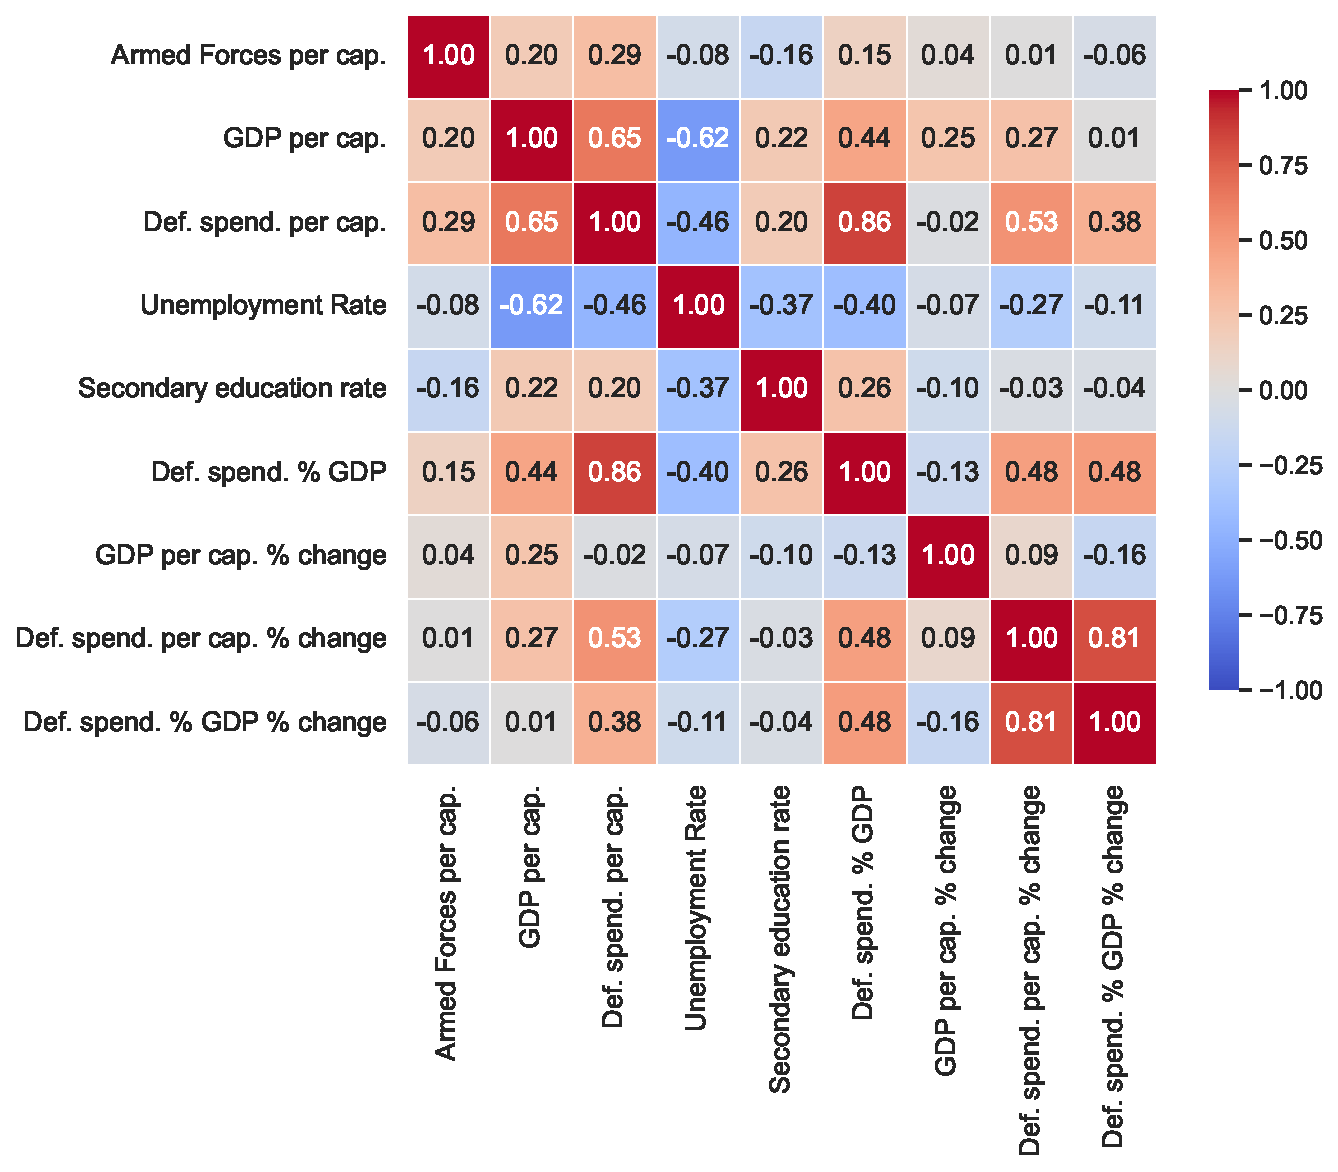
\includegraphics[width=1\textwidth]{images/correlation_heatmap.pdf}
    \label{fig:correlation_heatmap}
\end{figure}

As shown in Figure~\ref{fig:correlation_heatmap}, the correlation analysis revealed no single factor with a strong correlation to active military personnel numbers.
Active armed forces per capita were found to have weak to moderate positive correlations with GDP per 
capita (0.17), defence spending proportion of GDP (0.14) and defence spending per capita (0.29).
Weak negative correlations were observed with unemployment rate
(-0.08), secondary education attainment rate (-0.12) and defence spending proportion of GDP annual 
change (-0.11). These findings suggest that military size may grow as a country's economy improves 
and defence spending rises, while higher unemployment and education attainment rates may be related 
to reductions in military personnel.

Notable strong correlations of independent variables were found to be between defence expenditure per capita and 
defence expenditure as a proportion of GDP (0.85), and between their annual changes (0.80). 
This was unsurprising given that these variables are derived from defence spending. 
However, such large correlations may indicate multicollinearity, which could 
bias regression estimates and inflate standard errors. This meant that multicollinearity should be 
assessed before running the regression.

While the correlation analysis provides useful preliminary insight into the relationships between 
the variables, it does not isolate the direct effect of each variable. Therefore, a 
fixed-effects regression is used to estimate the conditional effects of the economic variables 
on active armed forces per capita, controlling for unobserved time-invariant heterogeneity 
across countries.

\subsection{Multicollinearity}

\begin{table}[ht]
\caption{Variance Inflation Factors (all variables)}
\small
\centering
\begin{tabularx}{\textwidth}{l r}
\toprule
\textbf{Variable} & \textbf{VIF} \\
\midrule
Unemployment rate & 1.95 \\
Secondary education rate & 1.27 \\
GDP per capita & 2.73 \\
Defence spending per capita & 6.00 \\
Defence spending \% of GDP & 4.93 \\
GDP per capita \% change & 1.35 \\
Defence spending per capita \% change & 4.28 \\
Defence spending \% GDP \% change & 4.43 \\
\bottomrule
\end{tabularx}
\label{tab:multicollinearity_full}
\end{table}

The initial results, displayed in Table~\ref{tab:multicollinearity_full}, showed moderate to high VIF values for defence spending per capita (6.00), 
defence spending as a percentage of GDP (4.93) and their respective annual percentage changes (4.28 and 4.43)
indicating the presence of multicollinearity. This is expected as these variables were highly correlated 
and capture similar underlying dynamics.
To mitigate 
this, variables defence spending per capita and its annual change were removed, and VIF values 
were calculated again.
It should be noted that a high VIF does not always justify the elimination of a variable;  
the exclusion should be theoretically motivated, for example if two variables measure 
the same underlying factor \parencite{obrien_caution_2007}. In this case, the 
exclusion of one of the two defence spending variables makes sense, as they are conceptually similar.

Table~\ref{tab:multicollinearity_reduced} reports the VIF values, excluding the possibly multicollinear 
cariables.
The VIF values reduced significantly, with defence spending's share of GDP now having 
1.93 and its annual change having 1.50. The observed reduction in multicollinearity motivated the 
estimation of two regression models: a full model including all variables and a reduced model 
excluding the highly collinear variables. This motivates a robustness check to ensure whether 
the findings of the models are stable or influenced by multicollinearity.

\begin{table}[ht]
\caption{Variance Inflation Factors (reduced variables)}
\small
\centering
\begin{tabularx}{\textwidth}{l r}
\toprule
\textbf{Variable} & \textbf{VIF} \\
\midrule
Unemployment rate & 1.89 \\
Secondary education rate & 1.23 \\
GDP per capita & 2.10 \\
Defence spending \% of GDP & 1.93 \\
GDP per capita \% change & 1.19 \\
Defence spending \% GDP \% change & 1.50 \\
\bottomrule
\end{tabularx}
\label{tab:multicollinearity_reduced}
\end{table}

\section{Regression analysis}

\subsection{Robustness check}

Two fixed-effects regression models were estimated to assess the robustness of the model, 
Table~\ref{tab:robustness} reports their summaries. 
The first was a base model, 
which included all variables, and the second was a reduced model with defence budget 
per capita and its annual change excluded, as these variables had exhibited multicollinearity 
with defence budget's proportion of GDP and its annual change.

\renewcommand{\arraystretch}{1.3}

\begin{table}[ht]
\small
\caption{Robustness check}
\centering
\resizebox{\textwidth}{!}{%
\begin{tabularx}{\textwidth}{>{\hsize=0.85\hsize\raggedright\arraybackslash}X 
                            >{\hsize=1\hsize\raggedright\arraybackslash}X 
                            >{\hsize=1\hsize\raggedright\arraybackslash}X}
\toprule
\textbf{Term} & \textbf{Base model} & \textbf{Reduced model} \\
\midrule
\multicolumn{3}{l}{\textit{Coefficient estimates}} \\
Unemployment rate & $-0.0041, p=0.3719$ & $-0.0013, p=0.7758$ \\
Secondary education attainment rate & $-0.0075, p=0.0001$ & $-0.0083, p=0.0001$ \\
GDP per capita & $-0.1653, p=0.2939$ & $0.2376, p=0.0867$ \\
Def. budget per capita & $0.3829, p=0.0000$ & - \\
Def. budget \% GDP & $-0.1110, p=0.0202$ & $0.0846, p=0.0053$ \\
GDP per capita \% change & $0.0008, p=0.6900$ & $-0.0009, p=0.6437$ \\
Def. budget per capita \% change & $-0.0014, p=0.0517$ & - \\
Def. budget \% GDP \% change & $-0.0001, p=0.8607$ & $-0.0013, p=0.0082$ \\
\addlinespace
\multicolumn{3}{l}{\textit{Model statistics}} \\
$R^2$ (within) & 0.2066 & 0.1200 \\
F-statistic (robust) & $F(8,245)=7.97, p<0.001$ & $F(6,247)=5.61, p<0.001$ \\
\bottomrule
\end{tabularx}
}
\label{tab:robustness}
\end{table}

The full model explained a larger proportion of the within-country variance 
$(R^2 = 0.2066\, \text{vs.} \,0.1200)$
and included a statistically significant variable, defence spending per capita, which had a positive 
relationship with the dependent variable. However, the multicollinearity between defence spending per 
capita and defence spending's share of GDP could undermine the stability and interpretability 
of the model. This was evidenced by the change in the sign of defence spending's percentage of GDP 
coefficient from negative to positive. Defence spending's share of GDP was expected to exhibit 
effects in the same direction as defence budget per capita, as they are derived from the same underlying 
measure of defence budgets. The opposing signs in the full model and the change of direction in the 
reduced model raised concerns of multicollinearity distorting the individual coefficient estimates.
These concerns were further supported by the change in statistical significance of the annual change in defence budget's share of GDP, which was not significant in the full model, but became significant in 
the reduced one.
These inconsistencies supported the decision to remove the collinear variables and favour the reduced 
one, which could be more stable and interpretable.

\subsection{Sensitivity analysis}

Table ~\ref{tab:sensitivity} shows the
three models that were estimated to analyse the effect of interpolated and filled educational attainment values.
The secondary educational attainment rate coefficients stayed consistently negative and statistically
significant across models. Additionally, other coefficients also remained with similar magnitudes. 
This means that using interpolated values does not meaningfully distort the 
relationship with the target variable. This is supported by the fact that the dummy variable for 
interpolated values in Model C is not statistically significant, suggesting no systematic 
differences in observations, where the education rate was interpolated or filled in. 

\renewcommand{\arraystretch}{1.2}

\begin{table}[ht]
\small
\caption{Sensitivity analysis models}
\centering
\resizebox{\textwidth}{!}{%
\begin{tabularx}{\textwidth}{>{\hsize=0.85\hsize\raggedright\arraybackslash}X 
                            >{\hsize=1\hsize\raggedright\arraybackslash}X 
                            >{\hsize=1\hsize\raggedright\arraybackslash}X 
                            >{\hsize=1\hsize\raggedright\arraybackslash}X}
\toprule
\textbf{Term} & \textbf{Model A (full)} & \textbf{Model B (excl. filled)} & \textbf{Model C (full + dummy)} \\
\midrule
\multicolumn{4}{l}{\textit{Coefficient estimates}} \\
Unemployment rate & $-0.0013, p=0.7758$ & $-0.0024, p=0.6276$ & $-0.0011, p=0.8205$ \\
Secondary education attainment rate & $-0.0083, p=0.0001$ & $-0.0069, p=0.0013$ & $-0.0084, p<0.0001$ \\
GDP per capita & $0.2376, p=0.0867$ & $0.1537, p=0.3107$ & $0.2878, p=0.0480$ \\
Def. budget \% GDP & $0.0846, p=0.0053$ & $0.1003, p=0.0021$ & $0.0882, p=0.0038$ \\
GDP per capita \% change & $-0.0009, p=0.6437$ & $-0.0009, p=0.6462$ & $-0.0014, p=0.4804$\\
Def. budget \% GDP \% change & $-0.0013, p=0.0082$ & $-0.0017, p=0.0008$ & $-0.0013, p=0.0073$ \\
Interpolation dummy & - & - & $-0.0299, p=0.2529$ \\
\addlinespace
\multicolumn{4}{l}{\textit{Model statistics}} \\
Number of observations & 285 & 262 & 285 \\
$R^2$ (within) & 0.1200 & 0.1135 & 0.1247 \\
F-statistic (robust) & $F(6,247)=5.6143, p<0.001$ & $F(6,224)=4.7800, p<0.001$ & $F(7,246)=5.0059, p<0.001$ \\
\bottomrule
\end{tabularx}
}
\label{tab:sensitivity}
\end{table}

Based on these results, Model C with full data, including interpolated and filled values, and a dummy 
variable flagging imputed values was chosen
as the preferred regression model. While imputed data could introduce noise or subtle bias
into regression estimates, this did not appear to be the case this time, as the interpolation dummy 
variable was found to be statistically insignificant. 
Nevertheless, Model C was adopted as it retains the full sample size while explicitly controlling 
for data quality variation, thereby increasing the robustness of the model.
Additionally, Model C had a marginally larger within-country 
$R^2$, than Model A (0.1247 vs 0.1200), meaning it explained the variation within countries 
slightly better, which again supported the decision to choose Model C.

\subsection{Final model}

The summary of the final model is reported in Table~\ref{tab:model_summary}.
The final fixed-effects regression model had a 0.1247 within-entity $R^2$, meaning it explained 
approximately 12.47\% of within-country variation in the logarithm of active armed forces per capita.
The robust/clustered F-statistic for the model was $F(7, 246)=2.3521, p=0.0242$, 
showing joint significance of the independent variables.
In other words, the model better explains the variation in the dependent variable than a model with 
only country-specific intercepts and no independent variables. 

\renewcommand{\arraystretch}{1.3}

% Model Summary Table
\begin{table}[htbp]
\caption{PanelOLS Estimation Summary}
\centering
\begin{threeparttable}
\begin{tabularx}{\textwidth}{@{}lX@{}}
\toprule
\textbf{Dep. Variable} & \texttt{Active Armed Forces per capita} \\
\textbf{Estimator} & PanelOLS \\
\textbf{No. Observations} & 285 \\
\textbf{Entities} & 32 \\
\textbf{Time Periods} & 9 \\
\textbf{Cov. Estimator} & Clustered \\
\midrule
\textbf{R-squared (Within)} & 0.1247 \\
\textbf{Log-likelihood} & 259.79 \\
\textbf{F-statistic (robust)} & 2.3521 \\
\textbf{P-value (F-stat)} & 0.0242 \\
\textbf{Distribution} & F(7, 246) \\
\midrule
\textbf{F-test for Poolability} & 70.146 \\
\textbf{P-value} & 0.0000 \\
\textbf{Distribution} & F(31, 246) \\
\textbf{Included effects} & Entity \\
\bottomrule
\end{tabularx}
\end{threeparttable}
\label{tab:model_summary}
\end{table}

Table~\ref{tab:final_model} reports the parameter estimates for the final model. 
Unemployment rate proved to be statistically insignificant $(-0.0011, p=0.9039)$, 
indicating that it may not substantially affect military labour supply in the sampled country and year subset.
Secondary education attainment rate exhibited a significant, modest negative relationship $(-0.0084, p=0.0424)$ 
with the dependent variable, meaning for every 1 percentage point increase in secondary education 
attainment rate, the active military size per capita decreased by approximately 0.84\%.
This negative relationship could be caused by multiple factors, for example, more educated individuals 
may consider their opportunities better in the civilian sector, while it could also be that countries 
with higher educational attainment rates have more technologically advanced armed forces, which require 
less manpower.

% Parameter Estimates Table
\begin{table}[htbp]
\caption{Parameter Estimates}
\centering
\begin{threeparttable}
\begin{tabularx}{\textwidth}{@{}Xrrrrrr@{}}
\toprule
\textbf{Variable} & \textbf{Coef.} & \textbf{Std. Err.} & \textbf{t-stat} & \textbf{p-value} & \textbf{CI Lower} & \textbf{CI Upper} \\
\midrule
Unemployment rate & -0.0011 & 0.0088 & -0.1208 & 0.9039 & -0.0185 & 0.0163 \\
Secondary education attainment rate & -0.0084 & 0.0041 & -2.0404 & 0.0424 & -0.0165 & -0.0003 \\
GDP per capita & 0.2878 & 0.2506 & 1.1484 & 0.2519 & -0.2058 & 0.7813 \\
Def. budget \% GDP & 0.0882 & 0.0379 & 2.3250 & 0.0209 & 0.0135 & 0.1629 \\
GDP per capita \% change & -0.0014 & 0.0016 & -0.8991 & 0.3695 & -0.0045 & 0.0017 \\
Def. budget \% GDP \% change & -0.0013 & 0.0007 & -1.7632 & 0.0791 & -0.0027 & 0.0001 \\
Education Dummy & -0.0299 & 0.0223 & -1.3412 & 0.1811 & -0.0739 & 0.0140 \\
\bottomrule
\end{tabularx}
\end{threeparttable}
\label{tab:final_model}
\end{table}

The logarithm of GDP per capita had a positive, but insignificant relationship $(0.2878, p=0.2519)$ 
with armed forces per capita. This could suggest that the state of the economy alone does not 
systematically influence the size of a county's active military. Wealthier countries may also
prioritize technology over manpower.
The annual change in GDP per capita was also found to be 
statistically insignificant $(-0.0014, p=0.3695)$,
indicating that short-term economic changes might not influence active military personnel size. 

Defence spending's share of GDP however, exhibited 
a significant and positive relationship $(0.0882, p=0.0209)$, meaning for each percentage point increase in defence spending's 
proportion of GDP, active military size per capita increased approximately 8.82\%.
The annual changes in defence spending's proportion of GDP proved to be an insignificant predictor
of active armed forces numbers $(-0.0013, p=0.0791)$. 
These findings could indicate that a higher baseline proportion of defence 
spending in GDP may signal long-term commitments to maintaining a large military, while short-term 
changes in the proportion may not directly predict a change in active military personnel. It could 
also be that short-term investments in defence spending were used for assets other than manpower.

It is important to note for the interpretation of these coefficients that the dependent variable was 
active military size per capita, meaning the coefficients reflect relative changes in active military personnel 
with respect to population size. Assuming a stable population, the reported percentage changes 
in active military size per capita can also be interpreted as approximate percentage changes in total 
active military size. However, in cases where population can vary notably, the per capita measure provides 
a more consistent comparison.